% ----------------------------------------------------------------------
%  Pracovní úkoly
% ----------------------------------------------------------------------
\section{Pracovní úkoly}

\begin{enumerate}
\item Pro tři vodorovné trubice s různými poloměry kruhového průřezu, které jsou opatřeny manometry, změřte závislost objemového průtoku Qv na úbytku statického tlaku \(\Delta p\) na vyšetřované délce trubice l ve směru proudění.

\item Sestrojte graf závislosti \(Qv = Qv(p).\)

\item Ze směrnice závislosti \(Qv = Qv(p)\) v oblasti laminárního proudění určete poloměr trubice.

\item Upravený poloměr dosaďte do vztahů pro výpočet Re a k.

\item Sestrojte graf závislosti k = k(Re), kde k je součinitel odporu trubice a Re je Reynoldsovo číslo. Do grafu vyneste teoretickou závislost pro laminární i turbulentní proudění.
\end{enumerate}

% ----------------------------------------------------------------------
%  Teoretická část
% ----------------------------------------------------------------------
\section{Teoretická část}

    Pro studium závislosti objemového průtoku \(Q_V\) na úbytku statického tlaku \(\Delta p\) použijeme aparaturu znázorněnou na obr. \ref{fig:schema}. Díky této závislosti určíme i oblasti laminárního a turbulentního proudění. Změnou rychlosti proudění vody v trubici s milimetrovou stupnicí se mění výška hladiny v manometru. Úbytek statického tlaku je dán vztahem

    \begin{equation}
        \Delta p = h\rho g,
    \end{equation}

    kde \(\rho\) je hustota kapaliny a \(g\) je místní tíhové zrychlení.

    \begin{figure}[h]
        \centering
        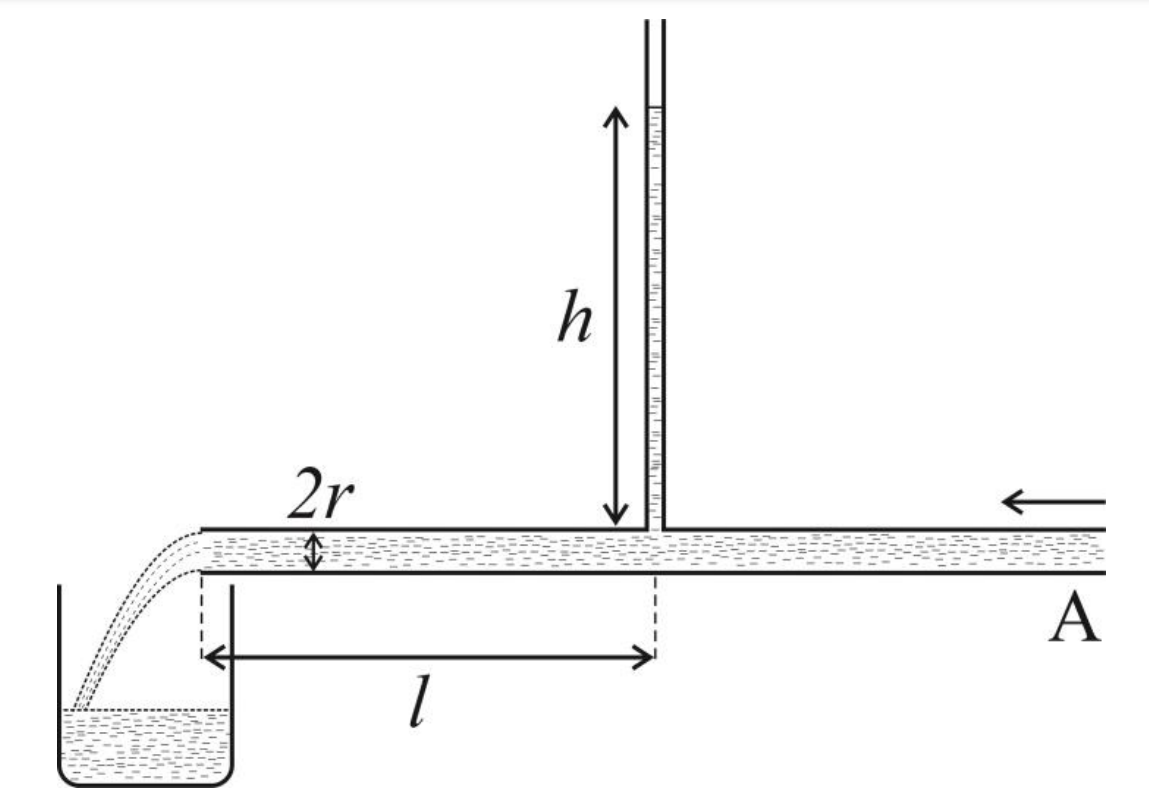
\includegraphics[width=0.5\linewidth]{01 - Studium proudění viskózní kapaliny trubicemi kruhového průřezu//Protokol//img/Schéma.png}
        \caption{Schéma zařízení.}
        \label{fig:schema}
    \end{figure}

    Objemový průtok je dán vztahem

    \begin{equation}
        Q_V = \frac{V}{t},
    \end{equation}

    kde \(V\) je objem kapaliny proteklé trubicí za čas \(t\).

    V oblasti laminárního proudění pro objemový průtok platí Poiseuillova rovnice

    \begin{equation}
        Q_V = \frac{\pi r^4}{8\eta l}\Delta p,
    \end{equation}

    kde \(r\) je vnitřní poloměr, \(l\) délka trubice a \(\eta\) dynamická viskozita proudící kapaliny.

    Proudění je laminární pokud nepřekročí kritickou hodnotu Reynoldsova čísla

    \begin{equation}
        Re = \frac{r\rho v_s}{\eta},
    \end{equation}

    kde \(v_s\) je střední rychlost proudění v trubici. Tato oblest je však určena pouze přibližně.

    Pro laminární proudění platí teoretický vztah

    \begin{equation}
        k = \frac{16}{Re},
    \end{equation}

    kde k je součinitel odporu trubice.

    Pro trubice s hladkými stěnami lze použít v případě turbulentního proudění lze použít vztah:

    \begin{equation}
        k \approx \frac{0,133}{\sqrt[4]{Re}}
    \end{equation}
% ----------------------------------------------------------------------
%  Výsledky a zpracování měření
% ----------------------------------------------------------------------
\section{Výsledky a zpracování měření}

\subsection{Laboratorní podmínky}

    Měření bylo prováděno za laboratorních podmínek uvedených v tabulce \ref{tab:lab_pod}. Pro naše měření je ale důležité, aby hodnoty (jako například teplota vody procházející  trubicí) byly co možná nejvíce podobné po celou dobu.

    \begin{table}[h]
        \centering
        \caption{Laboratorní podmínky}
        \label{tab:lab_pod}
        \begin{tabular}{|c|c|c|} 
        \hline
            t [°C] & p [hPa] & vlhkost [\%RH]  \\ 
        \hline
            22,9(40)   & 977,2(20)   & 34,7(25)            \\
        \hline
        \end{tabular}
    \end{table}

\subsection{Rozměry trubic}

    Vnitřní průměry trubic byly měřeny pomocí plastového posuvného měřidla. Udávaná přesnost je 0,05 mm, protože je ale měřidlo vyrobené z plastu a již lehce opotřebované, ve skutečnosti je přesnost nižší. V tabulce \ref{tab:prumery} jsou uvedeny výsledné průměry pro každou trubici (A, B a C). Každá trubice byla změřena třikrát.

    \begin{table}[h]
        \centering
        \caption{Vnitřní průměry trubic}
        \label{tab:prumery}
        \begin{tabular}{|c|c|c|c|} 
        \hline
            číslo měření & d_A / mm & d_B / mm & d_C / mm  \\ 
        \hline
            1            & 2,1(5)    & 2,7(5)    & 3,1(5)   \\
            2            & 2,1(5)    & 2,5(5)    & 3,0(5)   \\
            3            & 2,1(5)    & 2,7(5)    & 3,0(5)   \\ 
        \hline
            aritmetický průměr   & 2,1       & 2,6       & 3,0         \\
            standardní odchylka        & 0       & 0,1       & 0,1     \\
        \hline
        \end{tabular}
    \end{table}

    Vzdálenosti \(l\) každé trubice jsou uvedeny v tabulce \ref{tab:délky}. Tato vzdálenost byla změřena svinovacím metrem s přesností 0,5 mm.

    \begin{table}[h]
        \centering
        \caption{Délky trubic}
        \label{tab:délky}
        \begin{tabular}{|c|c|c|c|} 
        \hline
            číslo měření & d_A / mm & d_B / mm & d_C / mm  \\ 
        \hline
            1            & 251(5)    & 250(5)    & 202(5)   \\
            2            & 251(5)    & 250(5)    & 202(5)   \\
            3            & 251(5)    & 250(5)    & 202(5)   \\ 
        \hline
            výsledek     & 251(5)    & 250(5)    & 202(5)   \\
        \hline
        \end{tabular}
    \end{table}

\subsection{Teplota vody}

    Teplota vody byla změřena rtuťovým teploměrem třikrát - na začátku, v průběhu a na konci celého měření. Voda do trubice přitéká ze zásobníku na vodu, který je umístěn nad aparaturou. Je žádoucí, aby voda přitékala stále se stejnou teplotou, ale kvůli okolní teplotě lze předpokládat, že se v průběhu času postupně ohřívá.

    \begin{table}[h]
        \centering
        \caption{Teploty vody}
        \label{tab:teploty_vody}
        \begin{tabular}{|c|} 
        \hline
            t [°C]   \\ 
        \hline
            21,8(5)  \\
            22,1(5)  \\
            22,2(5)  \\
        \hline
        \end{tabular}
    \end{table}

    Na základě této teploty lze určit podle tabulek hustotu vody, která je 997,818 \SI{}{\kg\water\per\m\cubed\air}.

\subsection{Závislost objemového průtoku na úbytku tlaku}

    Závislost průtoku na tlaku byla měřena pomocí odměrného válce a ručních stopek. Množství vody a tedy její rychlost a změna tlaku byla regulována otočným kohoutem. Na začátku měření trubice byla stupnice manometru přibližně rozdělena do oblastí, kde dochází k laminárnímu proudění a kde ne. Díky to bylo možné naplánovat jednotlivá měření pro dostatek dat v laminární oblasti.

    V určité výšce manometru byl nastaven určitý tlak a poté změřen objem kapaliny proteklý trubicí za čas. V oblasti turbulentního proudění hladina vody v manometru neustále oscilovala, proto byla výška v tomto případě nastavena tak, aby hladina oscilovala kolem měřené hodnoty. Čas byl měřen pomocí stopek, kde počítáme s odchylkou reakční doby člověka.
    
    Chyba \(\Delta p\) byla vypočtena pomocí metody přenosu chyb podle

    \begin{equation}
        \sigma_\Delta_p = \sigma_h \rho g 
    \end{equation}

    Chyba objemového průtoku \(Q_V\) byla vypočtena také podle metody přenosu chyb jako

    \begin{equation}
        \frac{\sigma_Q__V}{\frac{V}{t}} = \sqrt{(\frac{\sigma_V}}{V})^2+(\frac{\sigma_t}{t})^2
    \end{equation}

\subsubsection{Trubice A}

    \begin{table}[h]
        \centering
        \caption{Trubice C}
        \label{tab:trubice C}
        \begin{tabular}{|c|c|c|c|c|}
        \hline
            h / cm   & V / ml  & t / s      & ∆p / Pa & Q / 10^{-6} m^3 s^−1  \\ 
        \hline
            23(0,05) & 200(10) & 20,72(20)  & 2251,4  & 0,965             \\
            22(0,05) & 200(10) & 21,50(20)  & 2153,5  & 0,930             \\
            21(0,05) & 200(10) & 21,59(20)  & 2055,6  & 0,926             \\
            20(0,05) & 200(10) & 22,38(20)  & 1957,7  & 0,894             \\
            19(0,05) & 200(10) & 23,34(20)  & 1859,8  & 0,857             \\
            18(0,05) & 200(10) & 23,81(20)  & 1761,9  & 0,840             \\
            17(0,05) & 200(10) & 24,60(20)  & 1664,1  & 0,813             \\
            16(0,05) & 200(10) & 25,19(20)  & 1566,2  & 0,794             \\
            15(0,05) & 200(10) & 26,91(20)  & 1468,3  & 0,743             \\
            14(0,05) & 200(10) & 26,97(20)  & 1370,4  & 0,742             \\
            13(0,05) & 200(10) & 28,12(20)  & 1272,5  & 0,711             \\
            12(0,05) & 200(10) & 28,00(20)  & 1174,6  & 0,714             \\
            11(0,05) & 200(10) & 28,41(20)  & 1076,7  & 0,704             \\
            10(0,05) & 200(10) & 29,10(20)  & 978,9   & 0,687             \\
            9(0,05)  & 200(10) & 29,22(20)  & 881,0   & 0,684             \\
            8(0,05)  & 200(10) & 31,03(20)  & 783,1   & 0,645             \\
            7(0,05)  & 200(10) & 33,44(20)  & 685,2   & 0,598             \\
            6(0,05)  & 200(10) & 37,78(20)  & 587,3   & 0,529             \\
            5(0,05)  & 200(10) & 42,69(20)  & 489,4   & 0,468             \\
            4(0,05)  & 200(10) & 51,06(20)  & 391,5   & 0,392             \\
            3(0,05)  & 200(10) & 69,81(20)  & 293,7   & 0,286             \\
            2(0,05)  & 200(10) & 105,82(20) & 195,8   & 0,189             \\
        \hline
        \end{tabular}
    \end{table}
    
% ----------------------------------------------------------------------
%  Diskuse výsledků
% ----------------------------------------------------------------------			
\section{Diskuse výsledků}

% ----------------------------------------------------------------------
%  Závěr
% ----------------------------------------------------------------------
\section{Závěr}
